\documentclass[tikz,convert={outfile=\jobname.svg}]{standalone}
\usepackage{tikz}
\usetikzlibrary{automata, positioning, arrows.meta, bending} % 'positioning' is helpful for arranging nodes

\begin{document}
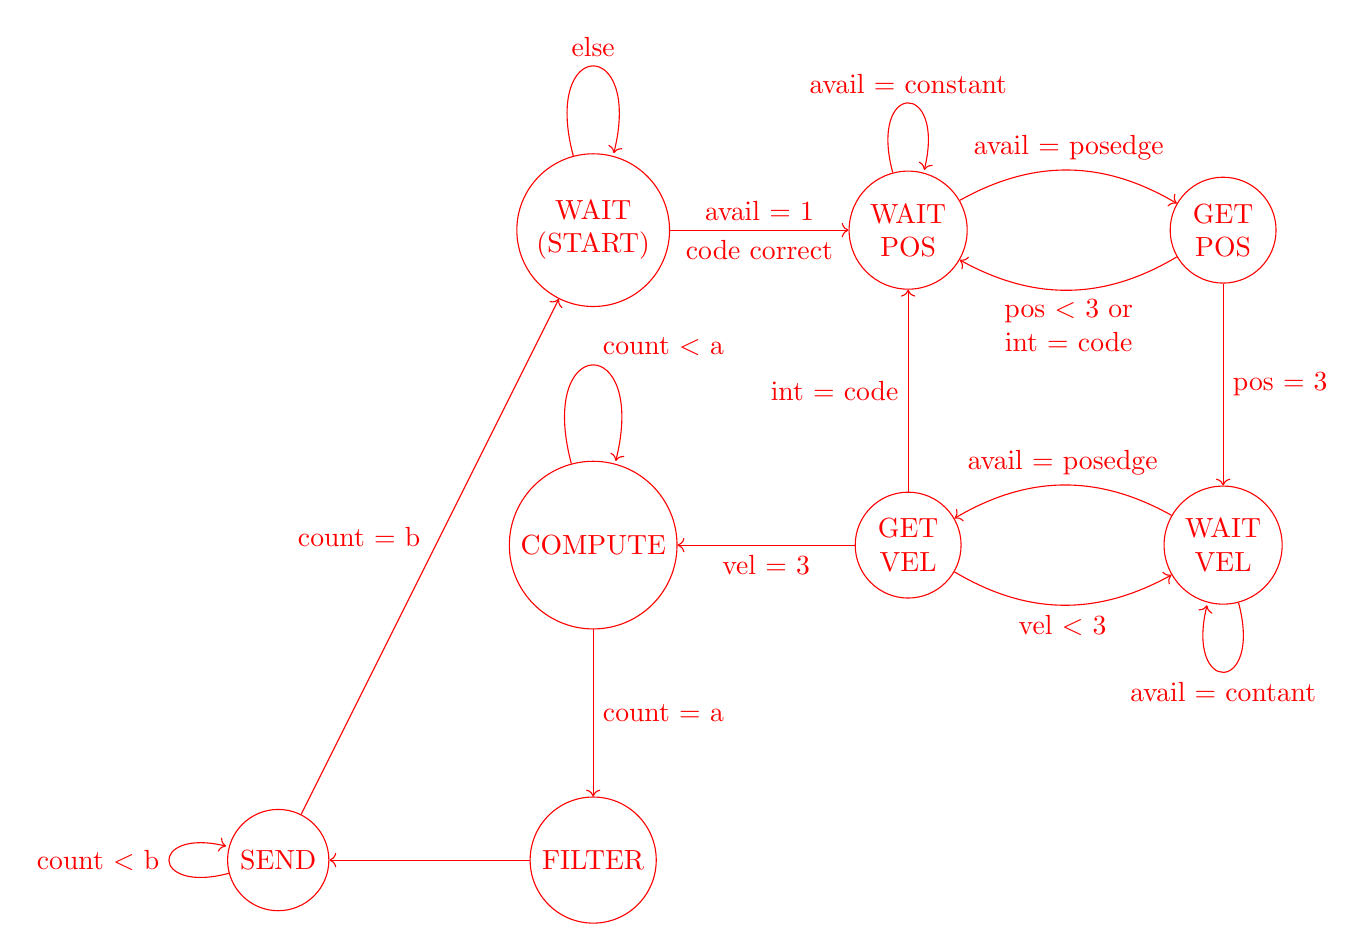
\begin{tikzpicture}[node distance=4cm, auto, state/.style={draw=red,shape=circle,text=red}, every node/.style={text=red}]

    % Define the states (nodes)
    \node[state, align=center] (s0) {WAIT\\(START)}; % Initial state 'q0'
    \node[state, right of=s0,align=center] (s1) {WAIT\\POS}; % Accepting state 'q1', positioned to the right of 'q0'
    \node[state, right of=s1,align=center] (s2) {GET\\POS};
    \node[state, below of=s2,align=center] (s3) {WAIT\\VEL};
    \node[state, left of=s3,align=center] (s4) {GET\\VEL};
    \node[state, left of=s4,align=center] (s5) {COMPUTE};
    \node[state, below of=s5,align=center] (s6) {FILTER};
    \node[state, left of=s6,align=center] (s7) {SEND};
    % Define the transitions (edges)
    \path[->, draw=red]
    (s0) edge node[above]{avail = 1} node[below]{code correct} (s1) %[draw = red]
    (s0) edge[loop above] node{else} (s0)
    (s1) edge[loop above] node{avail = constant} (s1)
    (s1) edge[bend left] node[above]{avail = posedge} (s2)
    (s2) edge[bend left] node[below, align=center]{pos $<$ 3 or\\int = code} (s1)
    (s2) edge node[right]{pos = 3}(s3)
    (s3) edge[loop below] node[below]{avail = contant} (s3)
    (s3) edge[bend right] node[above]{avail = posedge}(s4)
    (s4) edge[bend right] node[below]{vel $<$ 3}(s3)
    (s4) edge node{vel = 3} (s5)
    (s4) edge node[left]{int = code} (s1)
    (s5) edge[loop above] node[above right]{count $<$ a} (s5)
    (s5) edge node[right]{count = a}(s6)
    (s6) edge (s7)
    (s7) edge[loop left] node[left]{count $<$ b} (s7)
    (s7) edge node{count = b} (s0);

\end{tikzpicture}
\end{document}

